\documentclass{beamer}
\usepackage{mathtools}
\DeclarePairedDelimiter{\ceil}{\lceil}{\rceil}
\usepackage{algorithm}
\usepackage{algpseudocode}
\usepackage[english]{babel}
\usepackage[utf8]{inputenc}
\usetheme{Madrid}
\usecolortheme{dolphin}

\logo{\includegraphics[width=0.1\textwidth]{sdu_segl}}

\title{Interaktion og interaktionsdesign}
\author{Steven Gøhler}
\begin{document}
\begin{frame}
\titlepage
Redegør for forholdet mellem designets konceptuelle model og brugerens mentale model.
\end{frame}

\begin{frame}
  \frametitle{Overview}
  \tableofcontents
\end{frame}

\section{Brugerens mentale model}
\begin{frame}
\frametitle{Brugerens mentale model}
  \begin{columns}[T]
    \begin{column}{.5\textwidth}
	  \begin{itemize}
		\item Brugerens idé
		\item Hvordan produktet kommer til at virke
	    \item To type
	    \begin{itemize}
	      \item Hvordan bruges det
	      \item Hvordan fungerer det
	    \end{itemize}
	  \end{itemize}
    \end{column}
    \begin{column}{.5\textwidth}
      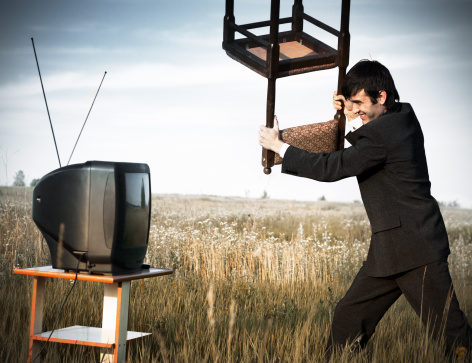
\includegraphics[width=\textwidth]{television.jpg}
    \end{column}
  \end{columns}
\end{frame}


\section{Konceptuel model}
\begin{frame}
\frametitle{Konceptuel model}
  \begin{columns}[T]
    \begin{column}{.5\textwidth}
	  \begin{itemize}
		\item Grundliggende idé
		\item Interaktion mellem funktioner
	    \item Fremvisning til brugeren
	    \item Brugerne kan lide den
	    \begin{itemize}
	      \item Gå videre til prototype design
	    \end{itemize}
	    \item Brugeren ikke tilfreds
	    \begin{itemize}
	      \item Tilbage til design start
	      \item Omstrukturering
	      \item Præsenter produktet igen
	    \end{itemize}
	  \end{itemize}
    \end{column}
    \begin{column}{.5\textwidth}
      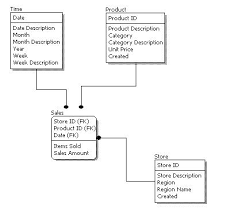
\includegraphics[width=\textwidth]{conceptual.png}
    \end{column}
  \end{columns}
\end{frame}

\section{Design}
\begin{frame}
  \frametitle{Design}
  \begin{columns}[T]
    \begin{column}{0.5\textwidth}
      \begin{itemize}
	    \item Konceptuelle og mentale model kan evt. udvikles samtidig
	    \item Brugerne skal involveres
	    \item Førstehåndsindtryk
	    \item Prototyper
      \end{itemize}  
    \end{column}
    \begin{column}{.5\textwidth}
      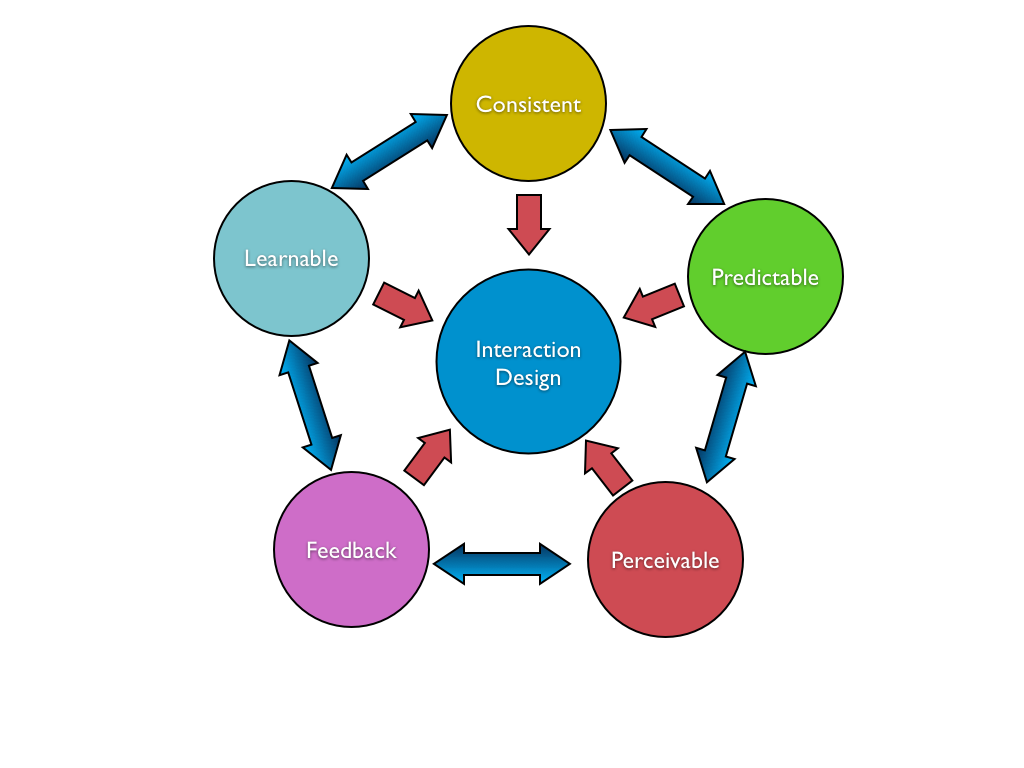
\includegraphics[width=\textwidth]{design.png}
    \end{column}
  \end{columns}
\end{frame}


\section{Prototype}
\begin{frame}
\frametitle{Prototype}
  \begin{columns}[T]
    \begin{column}{.5\textwidth}
	  \begin{itemize}
		\item Prototype testning af brugerne
		\item Bedste fra hver
		\item Hvad skal ændres?
		\item Tilbage til tegnebrættet
		\item Endelige produkt
	  \end{itemize}
    \end{column}
    \begin{column}{.4\textwidth}
      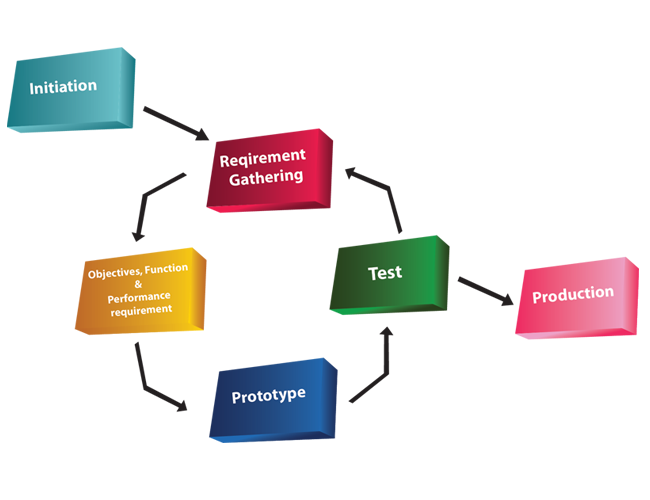
\includegraphics[width=\textwidth]{prototyping.png}
    \end{column}
  \end{columns}
\end{frame}


\end{document}